\newpage
\section{Task 2: Advanced normalisation}

Figure 2 below depicts an invoice for an order from a store.

\begin{figure}[H]
\centering
\caption{Pakoko Tax Invoice}
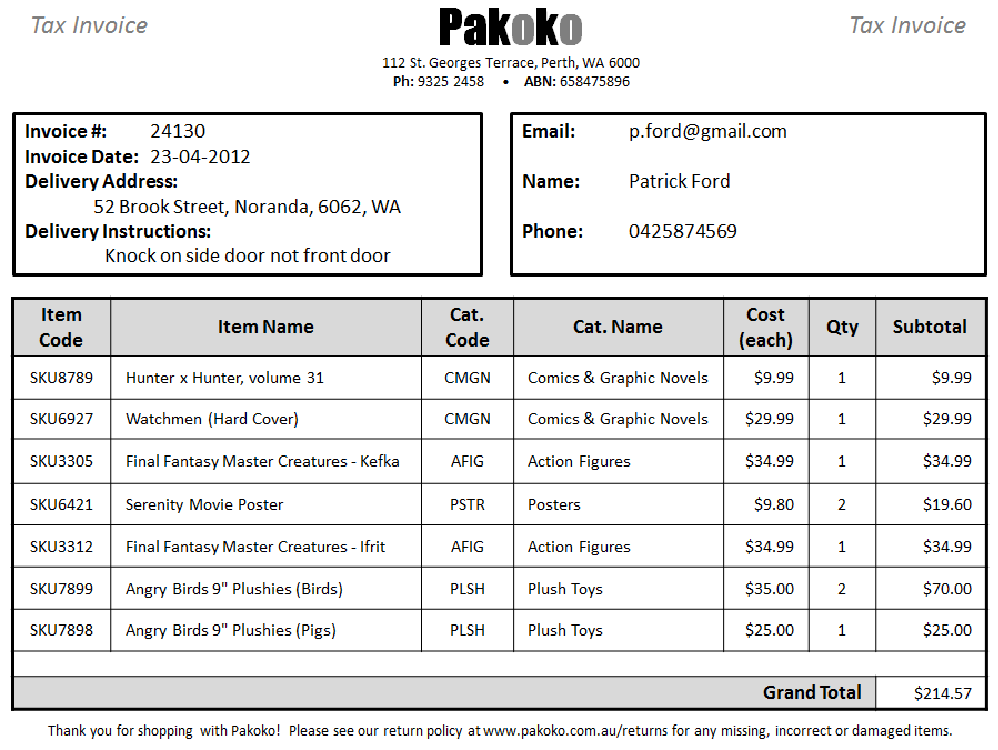
\includegraphics[scale=1]{./img/task2.pdf}
\end{figure}

\subsection*{Assumptions}

\begin{itemize}
\item The store identifies customers by their email address
\item Each item is only in one category
\item Item codes are unique per item, even if the items are in different categories
\item Invoice header and footer is static and is not stored in the database
\end{itemize}

\subsection{0NF: Unnormalised form}

R1 = (CustEmail, CustName, CustPhone, DeliveryAddress, DeliveryInstructions, \{Invoice\#, InvoiceDate, \{ItemCode, ItemName, CatCode, CatName, Cost, Qty\}\})

\subsection{1NF: First normal form}

\sout{R1 = (\textbf{\underline{CustEmail}}, CustName, CustPhone, DeliveryAddress, DeliveryInstructions, \{\textbf{\underline{Invoice\#}}, InvoiceDate, \{\textbf{\underline{ItemCode}}, ItemName, CatCode, CatName, Cost, Qty\}\})}
\\\\
R11 = (\textbf{\underline{CustEmail}}, CustName, CustPhone, DeliveryAddress, DeliveryInstructions)
\\\\
R12 = (\textbf{\underline{Invoice\#}}, InvoiceDate, \emph{CustEmail})
\\\\
R13 = (\textbf{\underline{\emph{Invoice\#}}}, \textbf{\underline{ItemCode}}, ItemName, CatCode, CatName, Cost, Qty)

\subsection{2NF: Second normal form}

R11 = (\textbf{\underline{CustEmail}}, CustName, CustPhone, DeliveryAddress, DeliveryInstructions)
\\\\
R12 = (\textbf{\underline{Invoice\#}}, InvoiceDate, \emph{CustEmail})
\\\\
\sout{R13 = (\textbf{\underline{\emph{Invoice\#}}}, \textbf{\underline{ItemCode}}, ItemName, CatCode, CatName, Cost, Qty)}
\\\\
R131 = (\textbf{\underline{\emph{Invoice\#}}}, \textbf{\underline{\emph{ItemCode}}}, Qty)
\\\\
R132 = (\textbf{\underline{ItemCode}}, ItemName, CatCode, CatName, Cost)

\subsection{3NF: Third normal form}

R11 = (\textbf{\underline{CustEmail}}, CustName, CustPhone, DeliveryAddress, DeliveryInstructions)
\\\\
R12 = (\textbf{\underline{Invoice\#}}, InvoiceDate, \emph{CustEmail})
\\\\
R131 = (\textbf{\underline{\emph{Invoice\#}}}, \textbf{\underline{\emph{ItemCode}}}, Qty)
\\\\
\sout{R132 = (\textbf{\underline{ItemCode}}, ItemName, CatCode, CatName, Cost)}
\\\\
R1321 = (\textbf{\underline{ItemCode}}, ItemName, \emph{CatCode})
\\\\
R1322 = (\textbf{\underline{CatCode}}, CatName)

\subsection{Named relations}

Customer = (\textbf{\underline{CustEmail}}, CustName, CustPhone, DeliveryAddress, DeliveryInstructions)
\\\\
Invoice = (\textbf{\underline{Invoice\#}}, InvoiceDate, \emph{CustEmail})
\\\\
InvoiceItem = (\textbf{\underline{\emph{Invoice\#}}}, \textbf{\underline{\emph{ItemCode}}}, Qty)
\\\\
Item = (\textbf{\underline{ItemCode}}, ItemName, \emph{CatCode})
\\\\
Category = (\textbf{\underline{CatCode}}, CatName)

\subsection{Physical E-R diagram}